\subsection*{Problema 28}

\textbf{Enunciado:} Calcular la integral:
\begin{equation*}
\int \dfrac{x + 5}{x^3 - 3x + 2} \, dx
\end{equation*}

\textbf{Solución:} 
Primero, factorizamos el denominador 
$P(x) = x^3 - 3x + 2$. 
Dado que $x = 1$ es una raíz evidente 
($1^3 - 3(1) + 2 = 0$), 
utilizamos división sintética o factorización 
por polinomios para obtener:
\begin{equation*}
x^3 - 3x + 2 = (x - 1)^2 (x + 2)
\end{equation*}

Planteamos la descomposición en 
fracciones parciales con factores 
repetidos y lineales:
\begin{multline*}
\dfrac{x + 5}{(x - 1)^2 (x + 2)} = \\
\dfrac{A}{x - 1} + \dfrac{B}{(x - 1)^2} + \dfrac{C}{x + 2}
\end{multline*}

Multiplicando ambos lados por el 
denominador común, obtenemos:
\begin{multline*}
x + 5 = A(x - 1)(x + 2) \\
+ B(x + 2) + C(x - 1)^2
\end{multline*}

Evaluamos en los valores clave para 
encontrar las constantes:
Si $x = 1$:
\begin{align*}
1 + 5 &= B(1 + 2) \implies 6 = 3B \implies B = 2
\end{align*}

Si $x = -2$:
\begin{align*}
-2 + 5 &= C(-2 - 1)^2 \implies 3 = 9C \implies C = \dfrac{1}{3}
\end{align*}

Si $x = 0$ y usando $B = 2$, $C = \dfrac{1}{3}$:
\begin{align*}
5 &= A(-1)(2) + 2(2) + \dfrac{1}{3}(-1)^2 \\
5 &= -2A + 4 + \dfrac{1}{3} \implies 2A = \dfrac{4}{3} \implies A = \dfrac{2}{3}
\end{align*}

Reemplazando los valores en la integral:
\begin{multline*}
\int \dfrac{x + 5}{x^3 - 3x + 2} \, dx = 
\int \left( \dfrac{2/3}{x - 1} + \dfrac{2}{(x - 1)^2} \right. \\
\left. + \dfrac{1/3}{x + 2} \right) dx
\end{multline*}

Integrando término a término:
\begin{align*}
&= \dfrac{2}{3}\ln|x - 1| - \dfrac{2}{x - 1} + \dfrac{1}{3}\ln|x + 2| + C
\end{align*}

Agrupando los términos logarítmicos:
\begin{align*}
&= \dfrac{1}{3}\ln\left| \dfrac{(x - 1)^2(x + 2)}{(x - 1)^3} \right| - \dfrac{2}{x - 1} + C
\end{align*}

La solución general de la integral es:
\begin{equation*}
\int \dfrac{x + 5}{x^3 - 3x + 2} \, dx = 
\dfrac{1}{3}\ln\left| \dfrac{x + 2}{x - 1} \right| - \dfrac{2}{x - 1} + C
\end{equation*}

\begin{figure}[H]
	\centering
	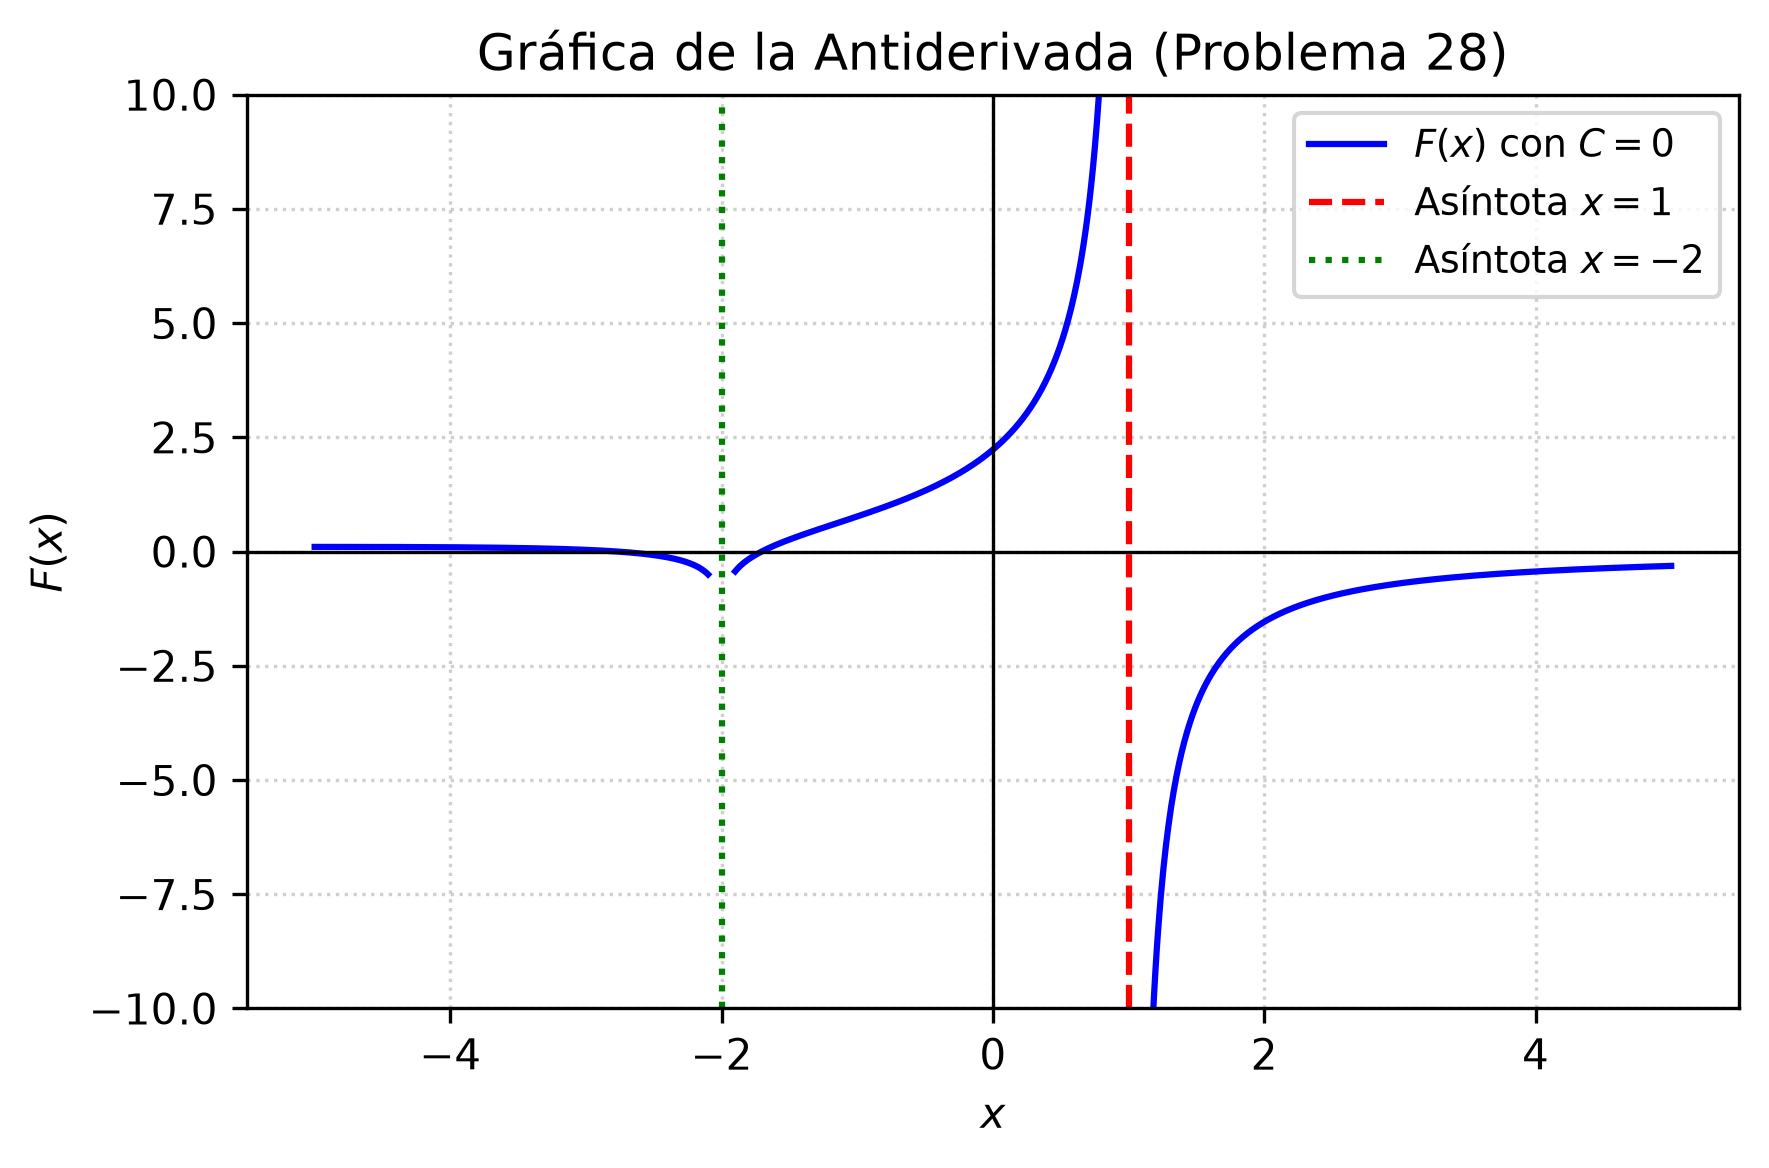
\includegraphics[width=\columnwidth]{semana_03/graficas/SEM03_P28_grafica.png}
	\caption{Representación gráfica de $f(x)$ y su antiderivada $F(x)$ evaluada para la constante de integración $C = 0$ (Problema 28).}
	\label{fig:problema28}
\end{figure}
